\documentclass[a4paper, 12pt]{article}	
\usepackage[top=2cm, bottom=2cm, left=2.5cm, right=2.5cm]{geometry}
\usepackage[utf8]{inputenc}
\usepackage{amsmath, amsfonts, amssymb}
\usepackage{graphicx}
\usepackage{float}
\usepackage[portuguese]{babel}
\usepackage{indentfirst}
\DeclareMathOperator{\sen}{sen}
\DeclareMathOperator{\arcsen}{arcsen}
\DeclareMathOperator{\arctg}{arctg}
\DeclareMathOperator{\tg}{tg}
\DeclareMathOperator{\cossec}{cossec}
\DeclareMathOperator{\arcsec}{arcsec}
\DeclareMathOperator{\arccossec}{arccossec}
\newcommand{\limite}{\displaystyle\lim}
\newcommand{\integral}{\displaystyle\int}
\newcommand{\somatorio}{\displaystyle\sum}
\newcommand{\produtorio}{\displaystyle\prod}
\title{ 
DOCUMENTAÇÃO \\ 
Final Fantasy}
\author{Guilherme Pereira Sarmento}
\date{30/08/2021} 
\begin{document}
\maketitle
\begin{itemize}
\item \textbf{Instuição}: UFMG

\item \textbf{Disciplina}: Programação e Desenvolvimento de Software I 

\item \textbf{Curso}: Física

\item \textbf{Professor}: Pedro Olmo Stancioli Vaz De Melo 
\end{itemize}

\section{Introdução}


  Essa documentação irá explicar o funcionamento do Trabalho Prático do curso de Programação e Desenvolvimento de Software I. Tal trabalho tinha como objetivo a realização, usando a biblioteca Allegro e a linguagem C, de um jogo com estruturas de RPG de turno semelhantes ao do primeiro Final Fantasy.

\subsection{Visão geral do jogo}

  No jogo, controlando o personagem criado por Andrzej Sapkowski, o bruxo Geralt de Rivia, devemos, através de um modo exploração, chegar até um tesouro. Porém, nesse caminho, orcs e murlocs, vindos diretamente do mundo de Azeroth, tentarão matar Geralt, sendo necessário, então, entrar em um modo de batalha de turnos com eles. Toda essa aventura do bruxo é acompanhada do clássico Kaiowas, do albúm CHAOS A.D. de 1993, tocando ao fundo.
  
  Ainda, também há um sistema de níveis implementado; quanto mais monstros mortos, maior será o nível jogador. Visto isso, o objetivo do jogo é chegar ao tesouro com o maior número de monstros mortos.
  
\subsection{Como jogar}

  O jogo começará, se não houver nenhum inimigo por perto, com Geralt no modo de exploração no canto inferior esquerdo da tela, de HP cheio, ou seja, igual a 100, e o objetivo, isto é o tesouro, estaticamente, no canto superior direito da tela. Para mover o bruxo pelo mapa usamos as ``setinhas" do teclado. 
  
  Se o personagem chegar muito perto do tesouro, o jogo acaba e aparece uma tela final de vitória. Ainda, caso o nível obtido seja o maior até então, a tela final sinalizará que um novo record foi obtido.
  
  Os monstros, por sua vez, são de dois tipos; os considerados fracos, os murlocs; e os considerados fortes, os orcs. Ao se inicializar o jogo, temos uma quantidade fixa de monstros (22) com HP cheio, ou seja, igual a 100 para os orcs e 70 para os murlocs, e cada respectiva posição desses será distruibuída ``aleatoriamente" pelo mapa.
  
   Se o personagem chegar muito perto de alguma dessas posições pré-estabelecidas, o jogo sairá de seu modo exploração e entrará no modo batalha. Caso seja a primeira vez do personagem nesse modo, Geralt começará o turno, caso contrário, será o monstro. 
   
   Para nosso personagem podemos escolher uma dentre três opções a cada turno, são elas o ataque normal, o ataque especial e a fuga. Para navegar entre essas opções usamos as teclas numéricas 1, 2 e 3, e para selicionar alguma pressionamos o ENTER.  
   
   O ataque normal retirará uma quantidade fixa de HP do monstro (35), o especial, por sua vez, retirará uma quantidade aleatória entre um valor menor do que o ataque normal e um maior (entre 20 e 65). Se o ataque for suficiente para acabar com o HP do monstro, o personagem voltará para o modo exploração ganhando um nível e o monstro será excluído do mapa. Por fim, caso a opção do bruxo seja fuga, teremos uma tentativa do personagem voltar para o modo exploração com uma probabilidade pré-definida (45 \%). Caso a fuga seja bem-sucedida o monstro não será morto, o que significa que ele ainda estará na mesma posição e que o bruxo não ganhará nenhum nível.
   
   Ao finalizar o turno do bruxo, isto é, ou o ataque já foi realizado ou a fuga foi mal-sucedida, será o turno do monstro. Este haverá somente um ataque pré-definido dependente do seu tipo, caso seja murloc, o ataque será um valor fixo menor (entre 12 e 17), e caso seja orc, será um valor fixo maior (entre 20 e 25). Tal ataque retirará HP do personagem, e, caso este chegue a zero, uma tela final de derrota será chamada.
   
\section{Detalhes da implementação do código}

  Tirando as definições globais, as implementações de bibiliotecas e as rotinas de inicialização do Allegro, o programa é dividido, basicamente, em três grandes blocos, a \textbf{função principal (int main)}, as \textbf{funções secundárias} e as \textbf{estruturas}.
  
  Para as estruturas, temos três: uma para o herói, uma para o monstro e outra que servirá de auxílio para desenhar os ataques na tela, i. e. para o ``bullet". 
  
  A struct do herói, contém as variáveis que o personagem irá possuir no modo exploração e batalha. Para o modo exploração temos inteiros que representam sua abcssisa e sua ordenada, e, para o modo batalha, há inteiros para ``segurar" a posição (x,y) do personagem para quando for voltar para o modo exploração; outro inteiro para representar qual será a ação do herói em seu turno (usado defines para cada tipo de ação); e,outro inteiro para saber se a execução foi ativada, isto é, se a tecla ENTER foi pressionada.
  
  A struct do monstro, analogamente a do herói, possui inteiros para sua posição (x,y), que serão sorteadas, para cada tipo monstro, no main, outro inteiro para o HP  e outro para armazenar qual o tipo do monstro (murloc ou orc). Para cada desse tipo foi criado um define correspondente.
  
  Para a struct do ``bullet", temos variáveis inteiras para a posição, outra para a velocidade do movimento do ataqu) e outra para o tamanho do ``bullet". Também temos uma variável do tipo ALLEGRO COLOR para a cor do ``bullet".
  
  Foi criado funções secundárias para inicilizar essa estruturas, como mostram as figuras abaixo:
  
\begin{figure}[H]
\centering
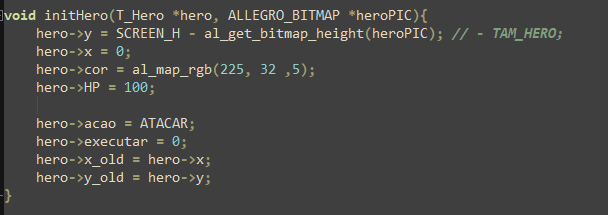
\includegraphics[scale=0.6]{init_hero.png}
\label{label1}
\end{figure}

\begin{figure}[H]
\centering
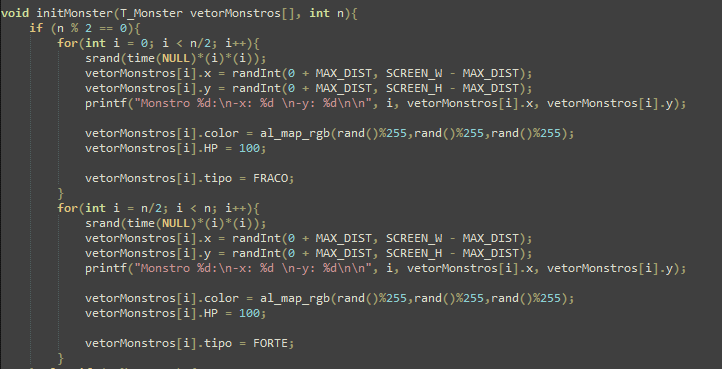
\includegraphics[scale=0.6]{init_monster.png}
\label{label2}
\end{figure}

\begin{figure}[H]
\centering
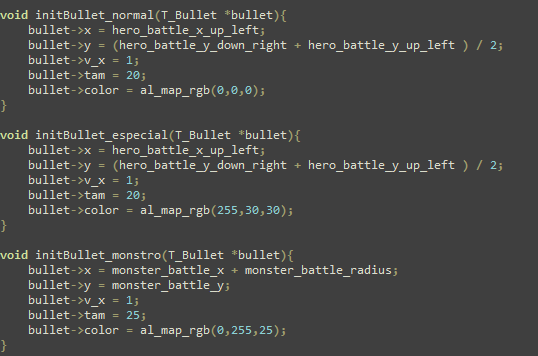
\includegraphics[scale=0.6]{init_bullet.png}
\label{label3}
\end{figure}

  Interessante notar que a função initMonster recebe como parâmetro um vetor do tipo monstro e o tamanho desse vetor, e ela irá inicializar para cada monstro nesse vetor as variáveis que são presentes na estrutura. No caso acima, metade dos monstros recebem o valor do tipo FRACO e a outra metade recebem o tipo FORTE e, perceba, que posição (x,y) é dada pela função randInt que retorna um número aleatório.
  
  Além disso, para inicializar o bullet, é necessário três funções. Isso ocorre pois são três tipos diferentes de ataque, dois do herói e um do monstro.
  
  A figura abaixo mostra a declaração e chamada das funções de inicialização das estruturas, no main:

\begin{figure}[H]
\centering
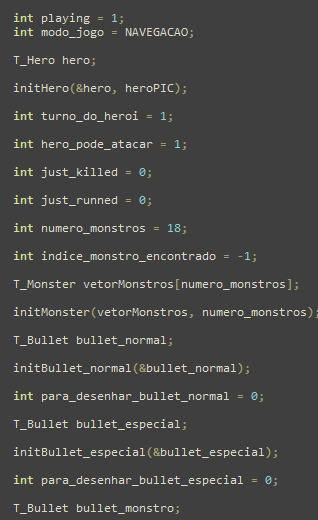
\includegraphics[scale=0.5]{variaveis_main.png}
\label{label4}
\end{figure}


  A primeira variável será reponsável por dizer se está acontecendo o jogo, caso positivo o while principal do main continuará sendo exectuado.  Já a segunda dirá qual será o modo de jogo, navegação ou batalha.
  
  Além de funções secundárias para a inicialização de estruturas também há funções para o desenho dos personagens e cenários, e para reprodução de sons.
  
  O funcionamento do while principal é baseado em eventos ALLEGRO do tipo tempo e do tipo tecla pressionada. Para cada evento de tempo, sempre verificamos primeiro se estamos no modo navegação ou no modo batalha; se nós encontramos no modo navegação, sempre é verificado se há algum monstro perto ou se já chegamos ao objetivo; caso encontramos no modo batalha variáveis auxiliares dizem de quem é o turno e se é para desenhar o ``bullet" ou não. Já se o evento for do tipo tecla pressionada, caso estejamos em exploração, será chamado uma função para processar as ``setinhas" do teclado; caso estejamos no modo batalha, outra função será chamada, que passando por referência o herói,  saberemos e qual é a ação a se realizar e se foi pressionada a tecla ENTER, então, chamaremos outra função para realizar a ação pedida, e mudaremos a variável de executar do hero para 0 (i.e. a tecla ENTER não foi mais pressionada).
  
  Depois do while principal, simplesmente iremos ler um arquivo txt, armazenar o valor de nível obtido na partida, e verificar se há algum outro valor maior do que obtido. Então, com a função de desenhar texto na tela da biblioteca allegro, escreveremos o requerido.
  
\end{document}	